

\section*{Appendix}

We present additional experimental results for the static hashing scenario. We vary the filled factor for each compared approaches and report the throughput for \formal{insert} and \formal{find} in Figure~\ref{fig:static:all:insert} and Figure~\ref{fig:static:all:search} respectively.
For insertion, it is expected that the overall performance drops as filled factor becomes larger across all approaches. 
\voter remains to be the second best solution behind \megakv except the \dsali dataset. As explained in Section~\ref{sec:exp:static}, the exception is due to the early termination of \cudpp once it detects insertion failures. \megakv achieves the best performance at the cost of high insertion failures (Tables~\ref{tab:fail:tw}-\ref{tab:fail:rand}). 

For \formal{find} operations, the performance remains constant for all approaches based on cuckoo hash. This is because it only requires to a fixed number of lookups to determine if a KV pair exists in the table. The throughput of \linear deteriorates for higher filled factors since it employs open addressing to resolve conflicts and one needs more lookups as the table fills up. This characteristic is also warp-inefficient as the workload for \formal{find} operation is not balanced.   

\begin{figure*}[t]
	\begin{minipage}{0.19\linewidth}\centering
		\includegraphics[width=\linewidth]{pic/static-upper/upper_insert_twitter.eps}
		\centerline{TW}
	\end{minipage}
	\hfill
	\begin{minipage}{0.19\linewidth}\centering
		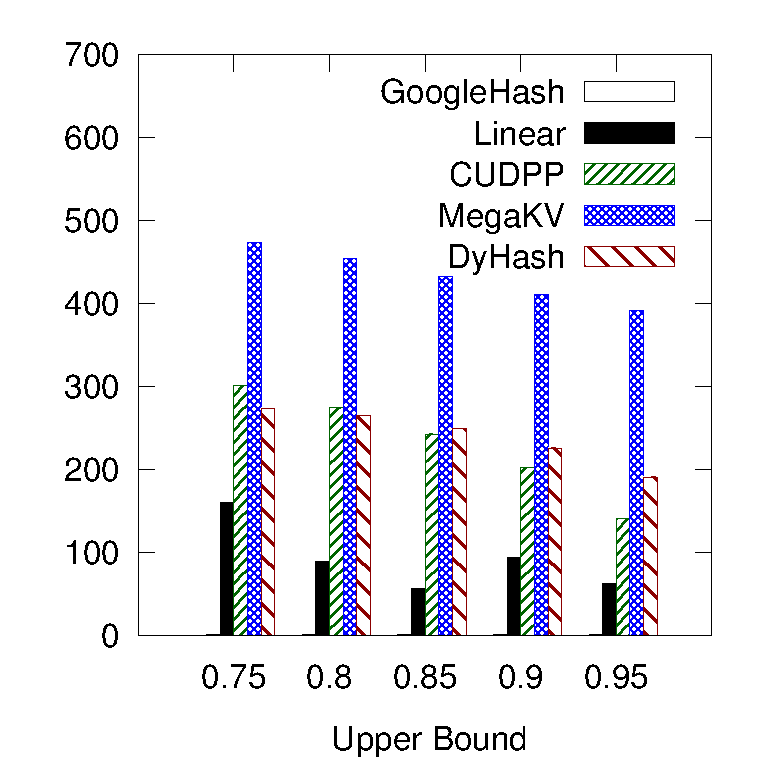
\includegraphics[width=\linewidth]{pic/static-upper/upper_insert_reddit.eps}
		\centerline{RE}
	\end{minipage}
	\hfill
	\begin{minipage}{0.19\linewidth}\centering
		\includegraphics[width=\linewidth]{pic/static-upper/upper_insert_tpch.eps}
		\centerline{LINE}
	\end{minipage}
	\hfill
	\begin{minipage}{0.19\linewidth}\centering
		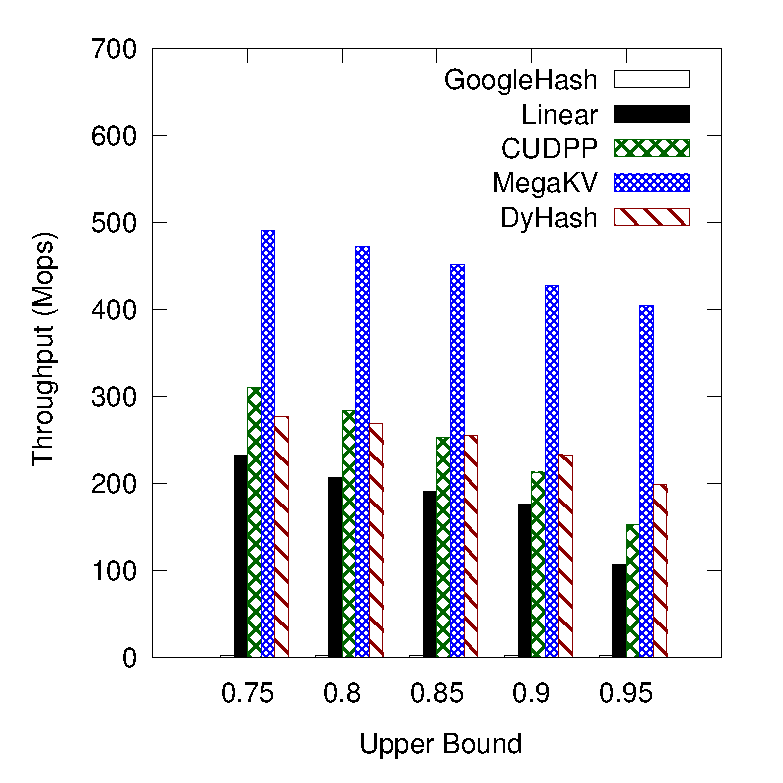
\includegraphics[width=\linewidth]{pic/static-upper/upper_insert_random.eps}
		\centerline{RAND}
	\end{minipage}
	\hfill
	\begin{minipage}{0.19\linewidth}\centering
		\includegraphics[width=\linewidth]{pic/static-upper/upper_insert_ali.eps}
		\centerline{COM}
	\end{minipage}
	\caption{Throughputs of insert for varying $\beta$.}
	\label{fig:static:all:insert}
\end{figure*}
\begin{figure*}[t]
	\begin{minipage}{0.19\linewidth}\centering
		\includegraphics[width=\linewidth]{pic/static-upper/upper_search_twitter.eps}
		\centerline{TW}
	\end{minipage}
	\hfill
	\begin{minipage}{0.19\linewidth}\centering
		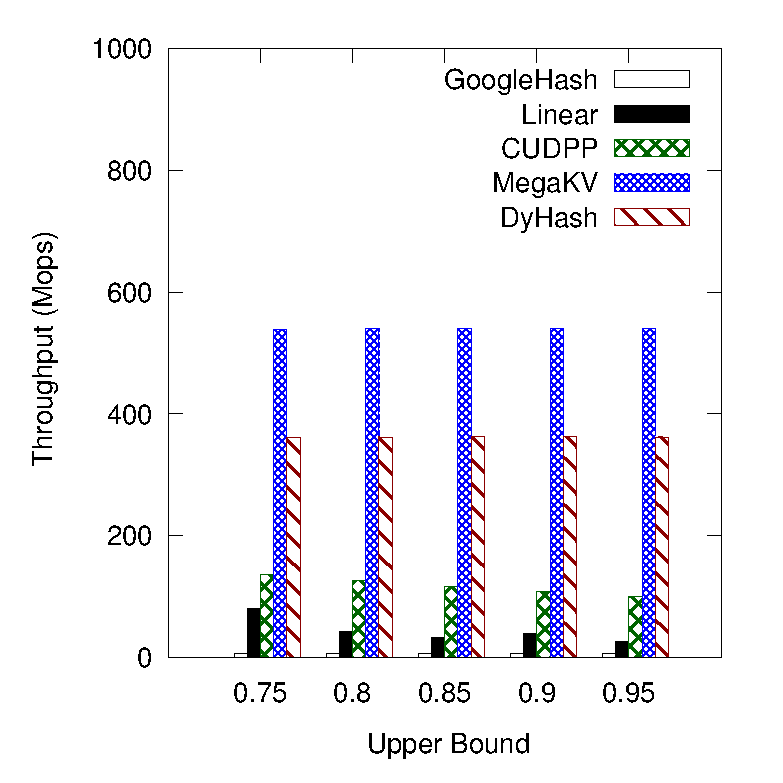
\includegraphics[width=\linewidth]{pic/static-upper/upper_search_reddit.eps}
		\centerline{RE}
	\end{minipage}
	\hfill
	\begin{minipage}{0.19\linewidth}\centering
		\includegraphics[width=\linewidth]{pic/static-upper/upper_search_tpch.eps}
		\centerline{LINE}
	\end{minipage}
	\hfill
	\begin{minipage}{0.19\linewidth}\centering
		\includegraphics[width=\linewidth]{pic/static-upper/upper_search_random.eps}
		\centerline{RAND}
	\end{minipage}
	\hfill
	\begin{minipage}{0.19\linewidth}\centering
		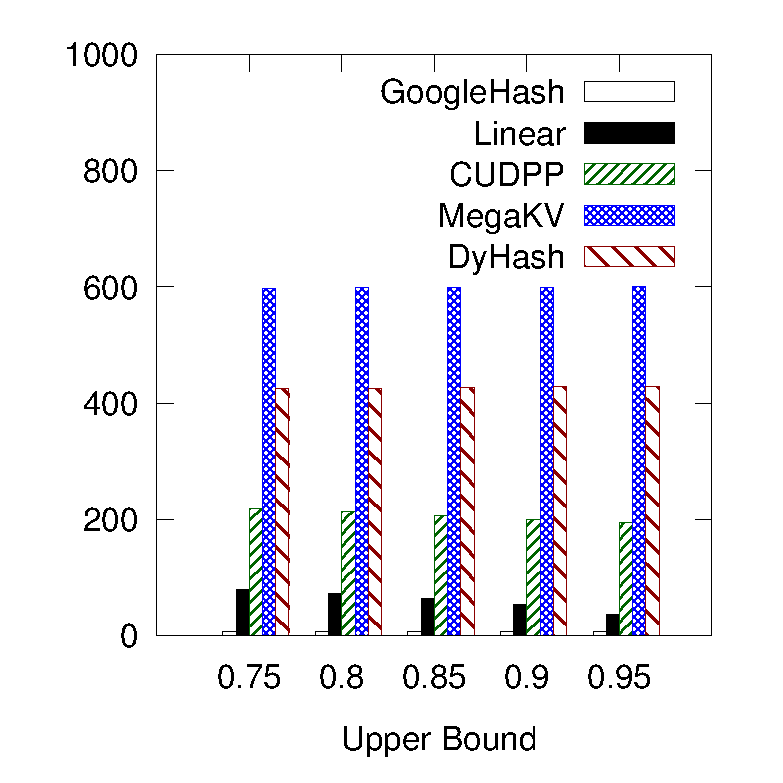
\includegraphics[width=\linewidth]{pic/static-upper/upper_search_ali.eps}
		\centerline{COM}
	\end{minipage}
	\caption{Throughputs of search for varying $\beta$.}
	\label{fig:static:all:search}
\end{figure*}

